
\subsubsection{$m_h$ and $\sigma_{Zh}$}
[recoil mass analysis, Fig.\ref{fig:RecoilMassLep250}, to be filled]
\begin{figure}
\begin{center}
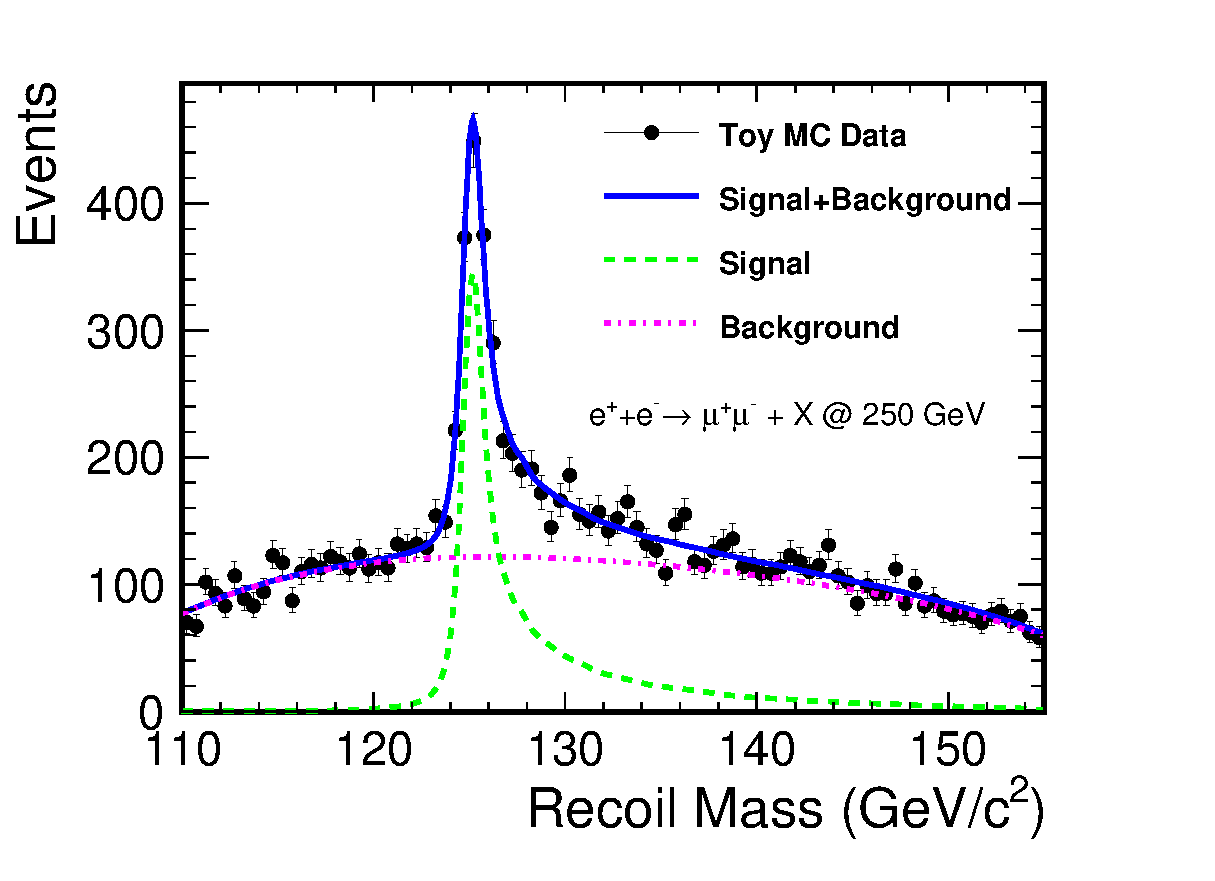
\includegraphics[width=0.85\hsize]{chapters/figures/RecoilMassLep250.eps}
\end{center}
  \caption{Recoil mass spectrum against
 $Z\to\mu^+\mu^-$ for signal $e^+e^-\to Zh$ and SM background 
  at 250 GeV \cite{Yan:2016xyx}.}
  \label{fig:RecoilMassLep250}
\end{figure}

\subsubsection{$\sigma_{\nu\bar{\nu}h}$ and $\sigma_{eeh}$}
[$W$-fusion and $Z$-fusion analyses, Fig.~\ref{fig:vvHbb}, to be filled]
\begin{figure}
%\begin{center}
\begin{tabular}[c]{c}
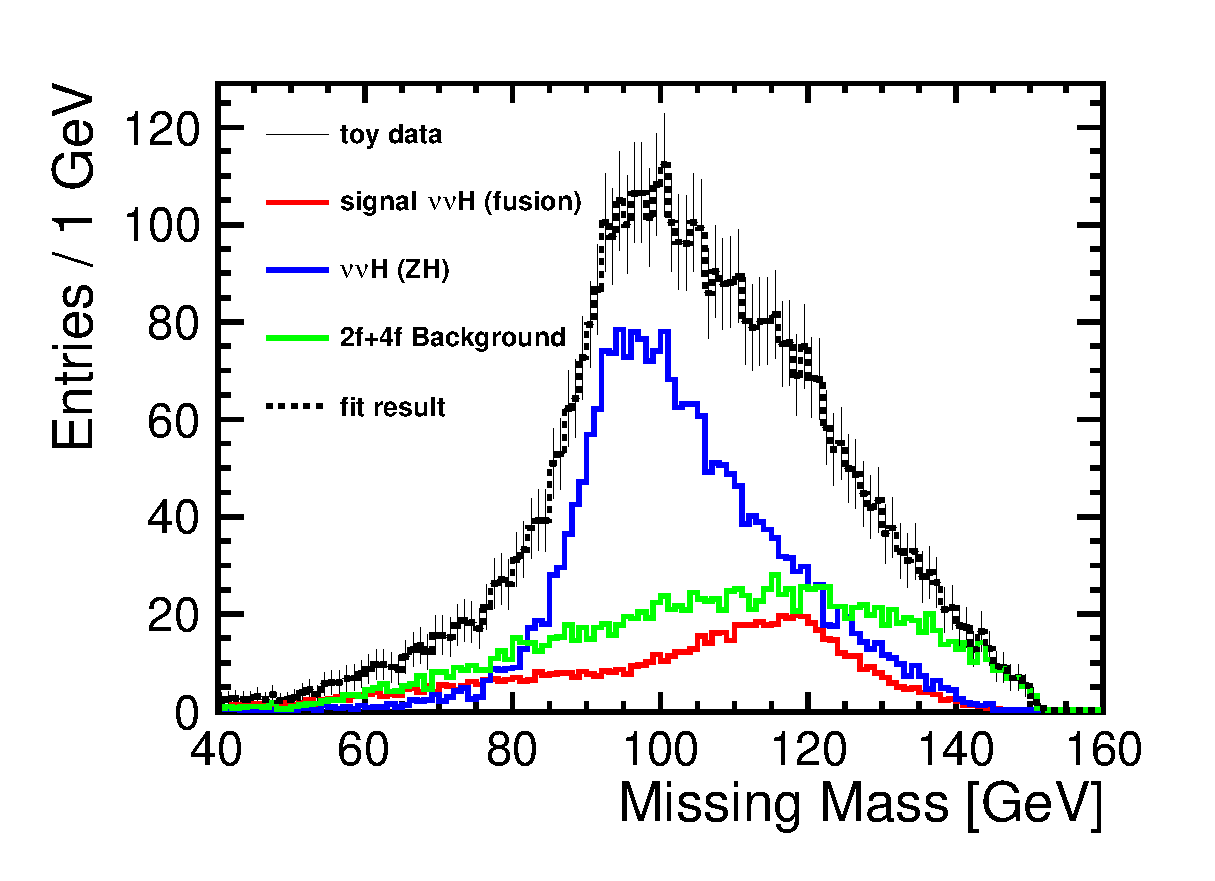
\includegraphics[width=0.85\hsize]{chapters/figures/vvH_MissingMass250.eps} \\
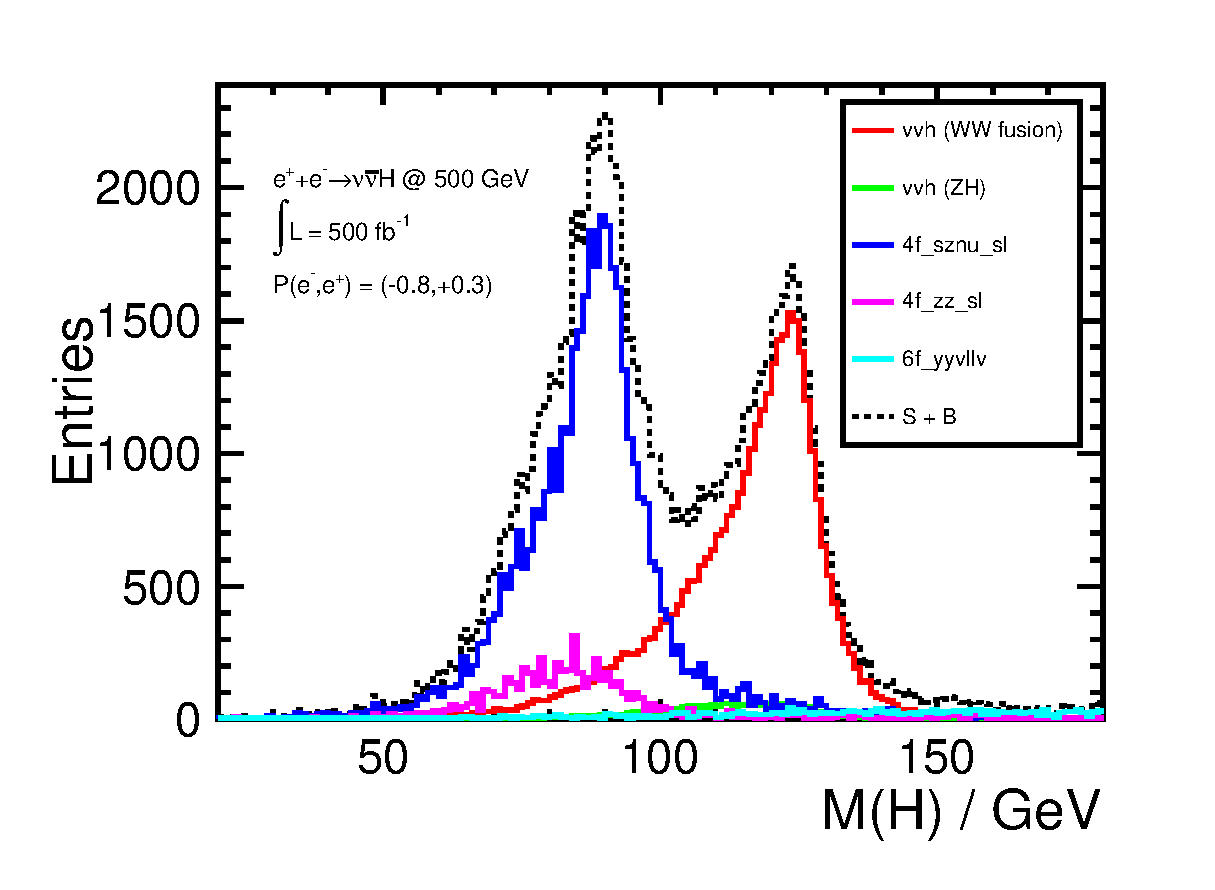
\includegraphics[width=0.85\hsize]{chapters/figures/vvH_MassH500.eps}
\end{tabular}
%\end{center}
  \caption{Missing mass spectrum (upper) and Higgs mass spectrum (lower) 
  for the signal $e^+e^-\to\nu\bar\nu h, h\to b \bar{b}$ and the SM background 
  at 250 GeV and 500 GeV respectively \cite{H2bb1,H2bb2}.}
  \label{fig:vvHbb}
\end{figure}

\subsubsection{$\mathrm{BR}(h\to b\bar{b}/c\bar{c}/gg)$}
[Fig.~\ref{fig:qqHbbccgg250}, to be filled]
\begin{figure*}
\begin{center}
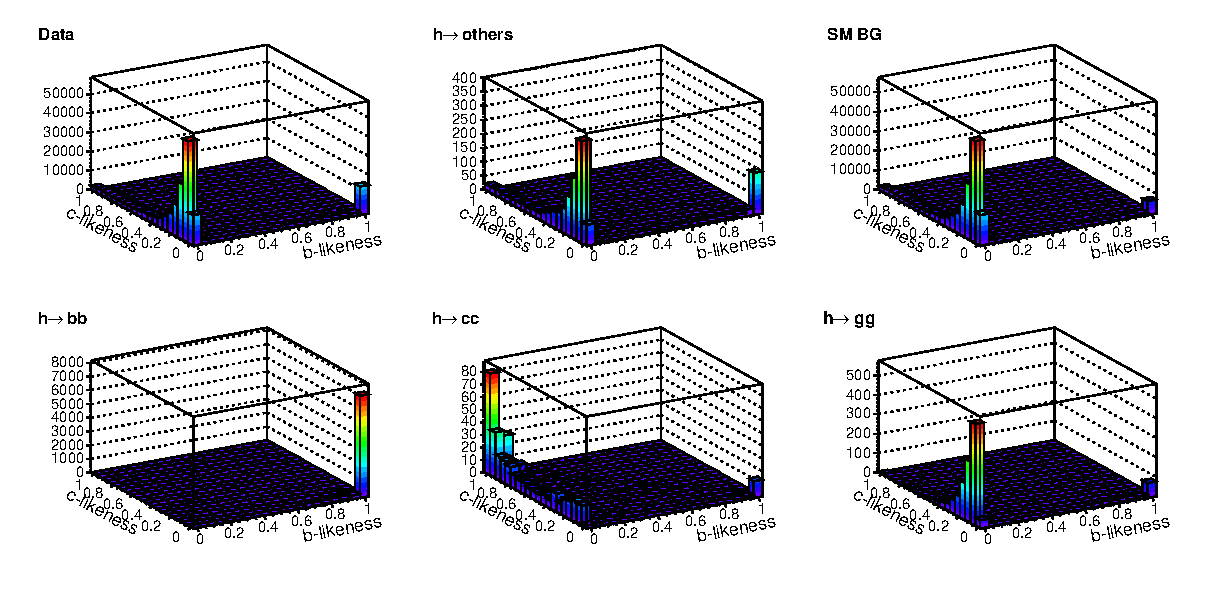
\includegraphics[width=0.85\hsize]{chapters/figures/qqh_bbccgg_template_250.eps}
\end{center}
  \caption{Template of b-likeliness versus c-likeness for signal $h\to b\bar{b}/c\bar{c}/gg$
  (bottom left/middle/right),
and for all events / $h\to others$ / SM background (top left/middle/right).}
  \label{fig:qqHbbccgg250}
\end{figure*}

\subsubsection{$\mathrm{BR}(h\to WW^*/ZZ^*)$}
[Fig.~\ref{fig:vvHWW500}, to be filled]
\begin{figure}
\begin{center}
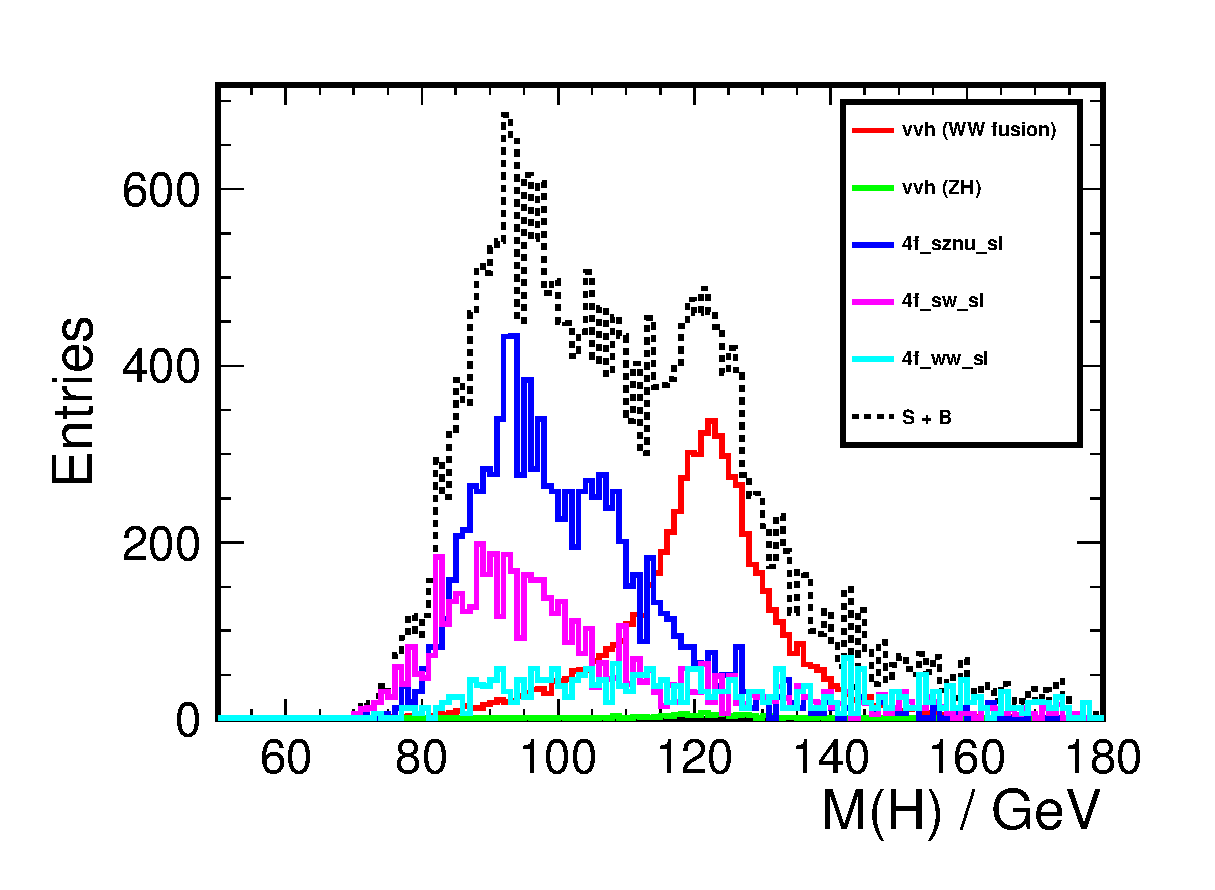
\includegraphics[width=0.85\hsize]{chapters/figures/vvH_WW4j500_MassH.eps}
\end{center}
  \caption{Higgs mass spectrum for the signal $e^+e^-\to\nu\bar\nu h, h\to WW^{*}$
  and $WW^{*}\to 4-jets$, and the SM background 
  at 500 GeV \cite{H2WW500}.}
  \label{fig:vvHWW500}
\end{figure}

\subsubsection{$\mathrm{BR}(h\to \tau^+\tau^-/\mu^+\mu^-)$}
[Fig.~\ref{fig:qqHtautau250}, to be filled]
\begin{figure}
\begin{center}
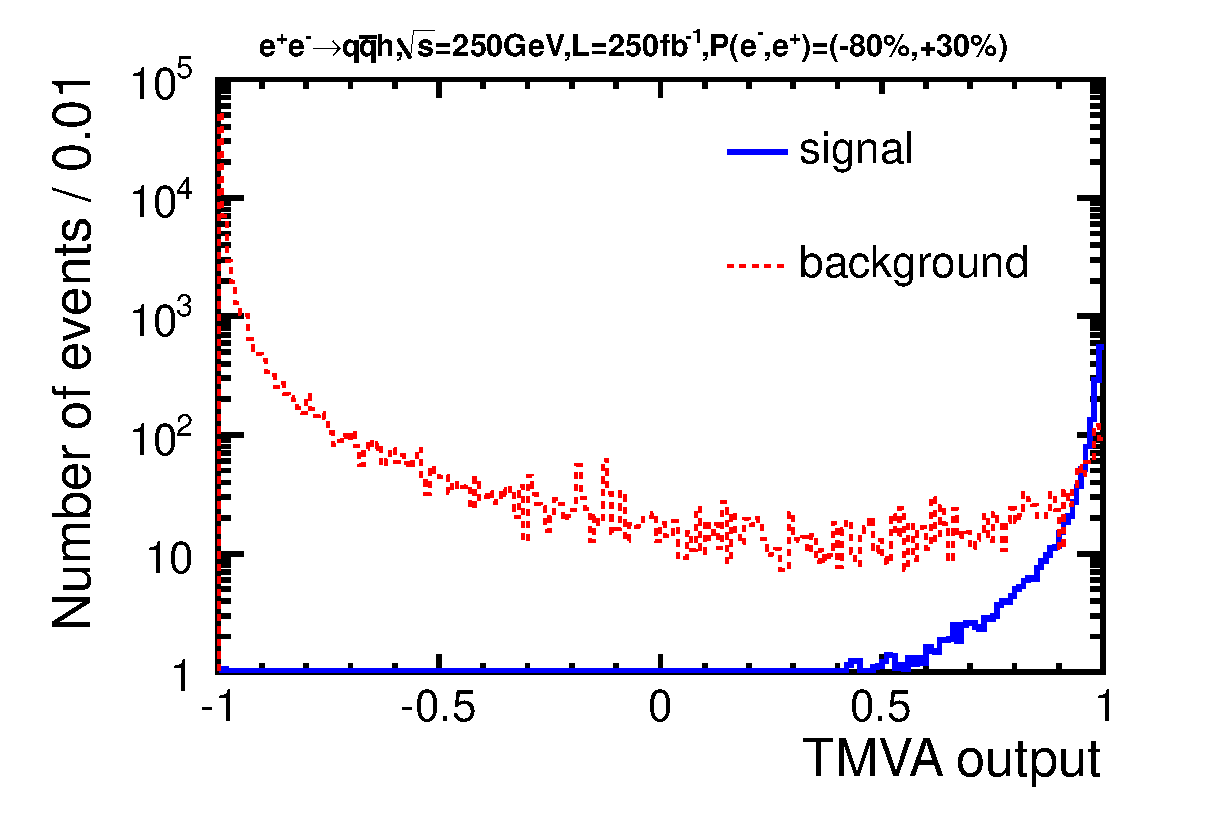
\includegraphics[width=0.85\hsize]{chapters/figures/ZH_qqtautau250_TMVA.eps}
\end{center}
  \caption{MVA output for the signal $e^+e^-\to q\bar{q} h, h\to\tau^+\tau^-$
 and the SM background at 250 GeV \cite{H2tautau250}.}
  \label{fig:qqHtautau250}
\end{figure}

\subsubsection{$\mathrm{BR}(h\to \mathrm{invisible/exotic})$}
[invisible analysis, Fig.\ref{fig:qqHinv250}, to be filled]
\begin{figure}
\begin{center}
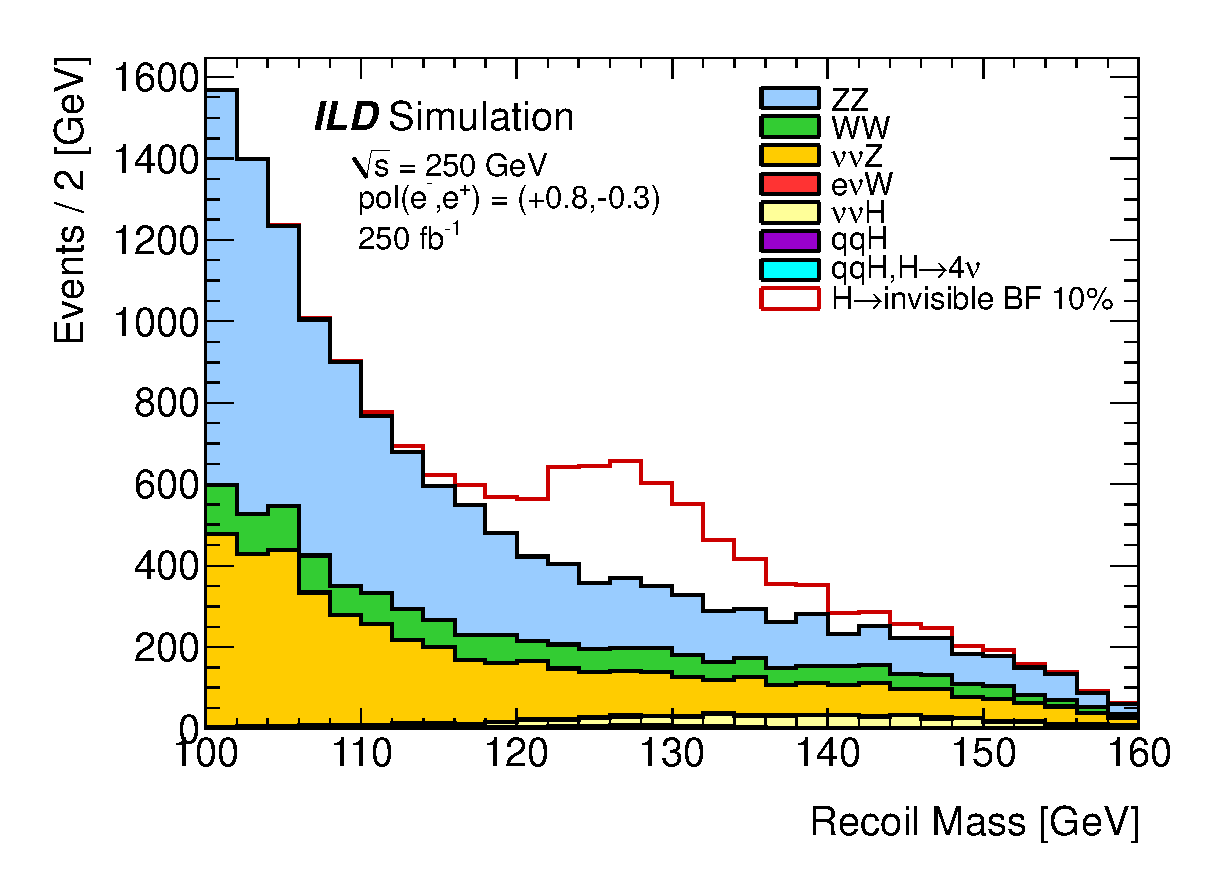
\includegraphics[width=0.85\hsize]{chapters/figures/ZH_qqinv250_right.eps}
\end{center}
  \caption{Recoil mass spectrum against
 $Z\to q\bar{q}$ for signal $e^+e^-\to Zh, h\to invisible$ assuming $BR(h\to invisible)=10\%$
  and SM background  at 250 GeV \cite{H2inv250}.}
  \label{fig:qqHinv250}
\end{figure}


\subsubsection{Higgs CP Properties}
[Fig.~\ref{fig:qqHtautauCP}, to be filled]
\begin{figure}
\begin{tabular}[c]{c}
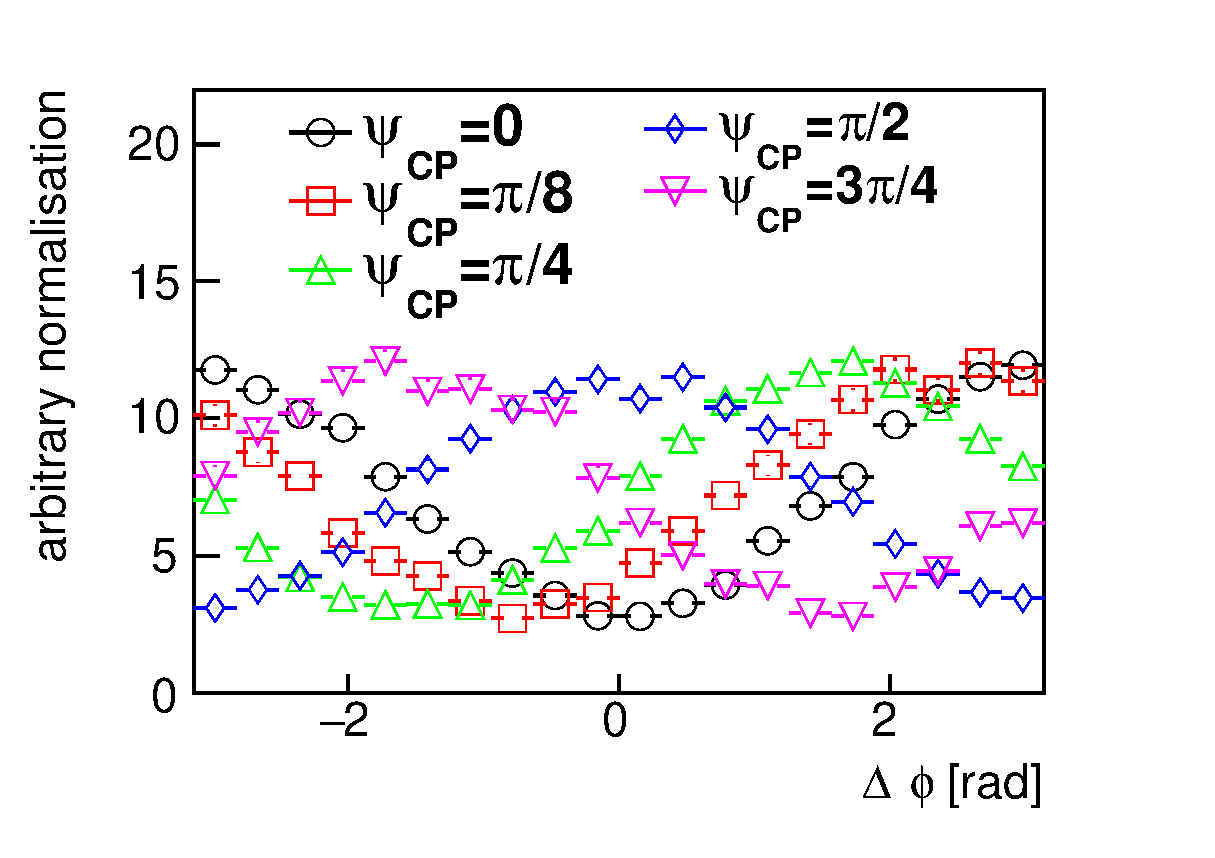
\includegraphics[width=0.85\hsize]{chapters/figures/ZH_qqtautau250_CP1.eps} \\
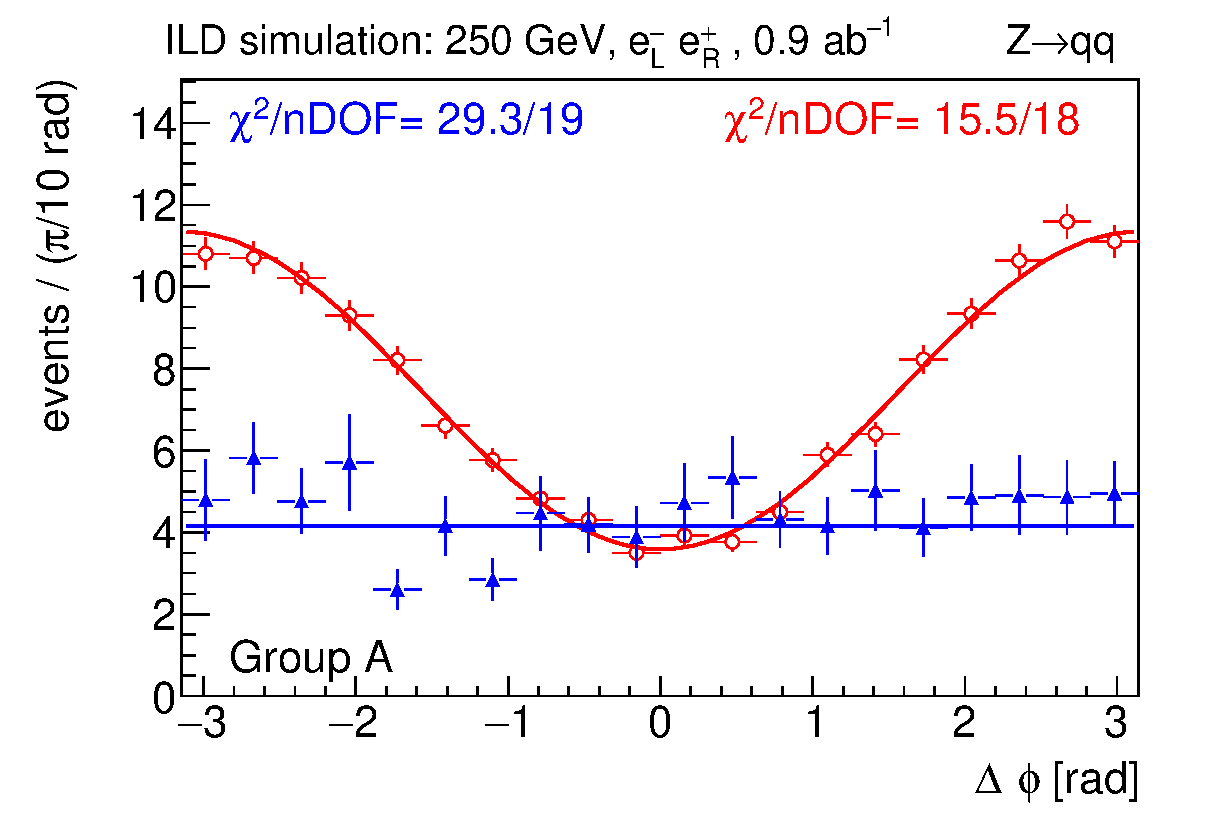
\includegraphics[width=0.85\hsize]{chapters/figures/ZH_qqtautau250_CP2.eps}
\end{tabular}
  \caption{Upper: $\Delta\phi$ distributions at MC Truth level for different 
  values of $\Phi_{CP}$ for the signal $e^+e^-\to q\bar{q} h, h\to\tau^+\tau^-$ at 250 GeV;
  Lower: reconstructed $\Delta\phi$ distributions after all cuts in the dominant category
  for the SM signal (in red) and the SM background (blue) respectively \cite{H2tautauCP}.}
  \label{fig:qqHtautauCP}
\end{figure}


\subsubsection{Angular Analyses for Anomalous $HVV$ Couplings}
[Fig.~\ref{fig:ZHanomHVV1} and~\ref{fig:ZHanomHVV2}, to be filled]
\begin{figure}
\begin{tabular}[c]{c}
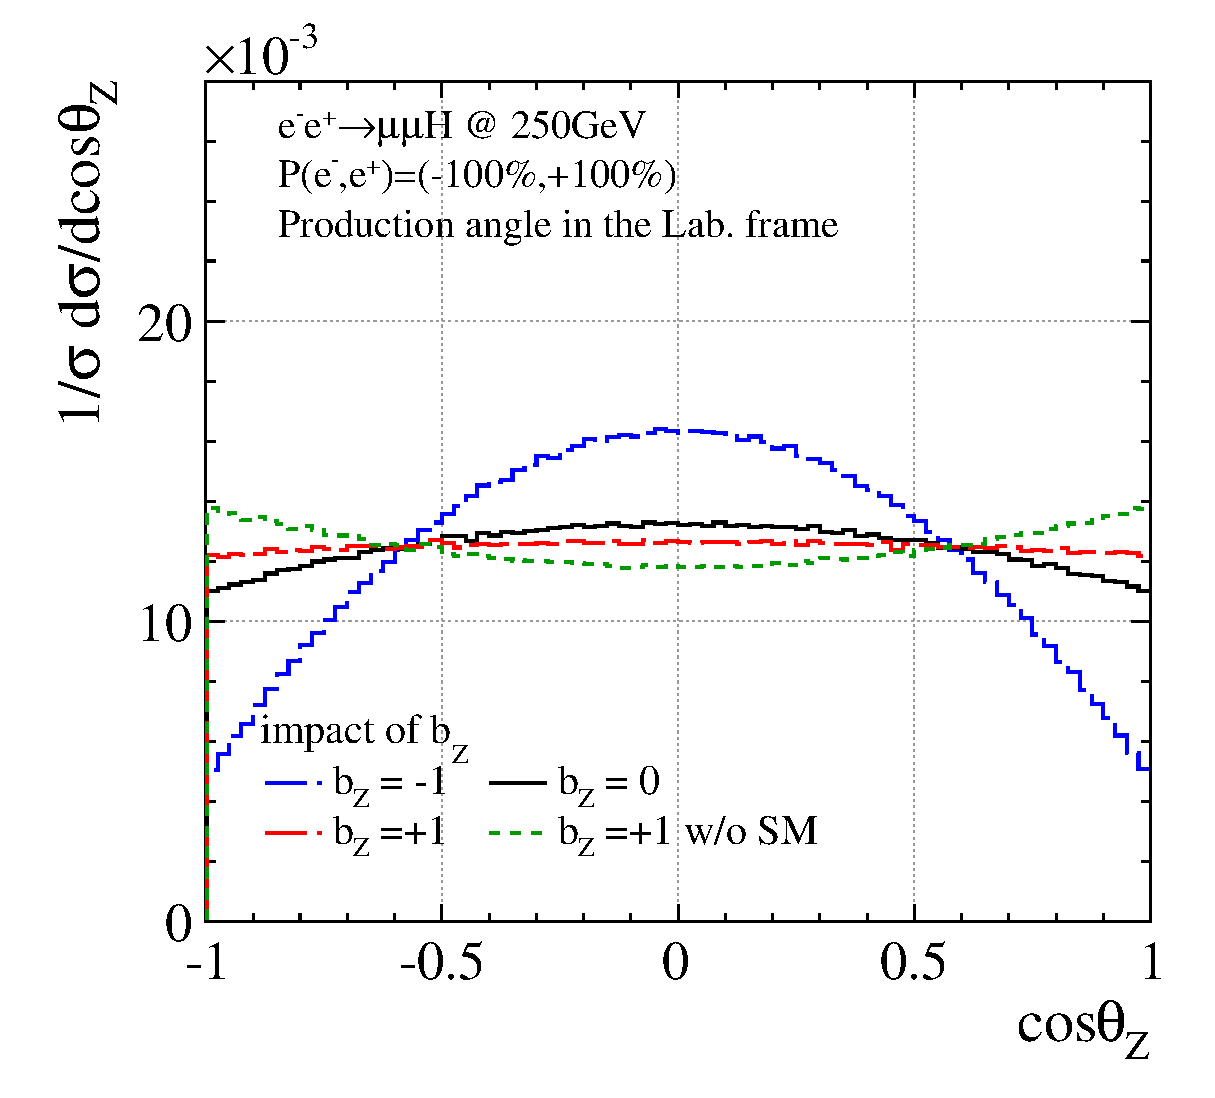
\includegraphics[width=0.85\hsize]{chapters/figures/ZH_anomHVV250_b.eps} \\
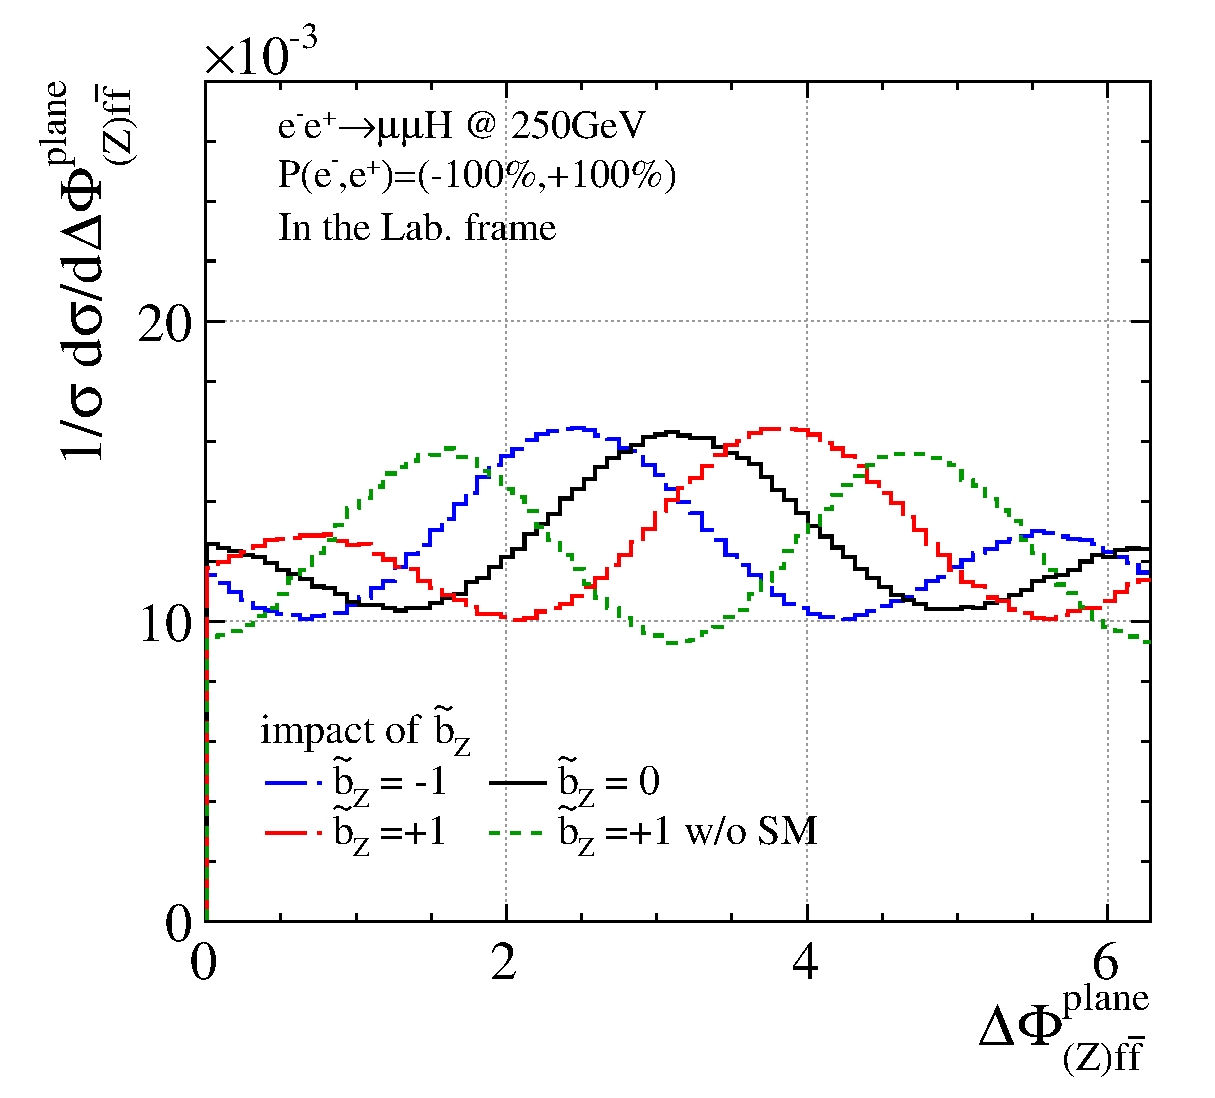
\includegraphics[width=0.85\hsize]{chapters/figures/ZH_anomHVV250_bt.eps} 
\end{tabular}
  \caption{Upper (lower): $\cos\theta_Z$ ($\Delta\Phi$) distributions at MC Truth level for different 
  values of anomalous coupling $b$ ($\tilde{b}$) 
  for the signal $e^+e^-\to \mu^+\mu^- h, h\to everthing$ at 250 GeV;
  \cite{anomHVV}.}
  \label{fig:ZHanomHVV1}
\end{figure}

\begin{figure*}
\begin{center}
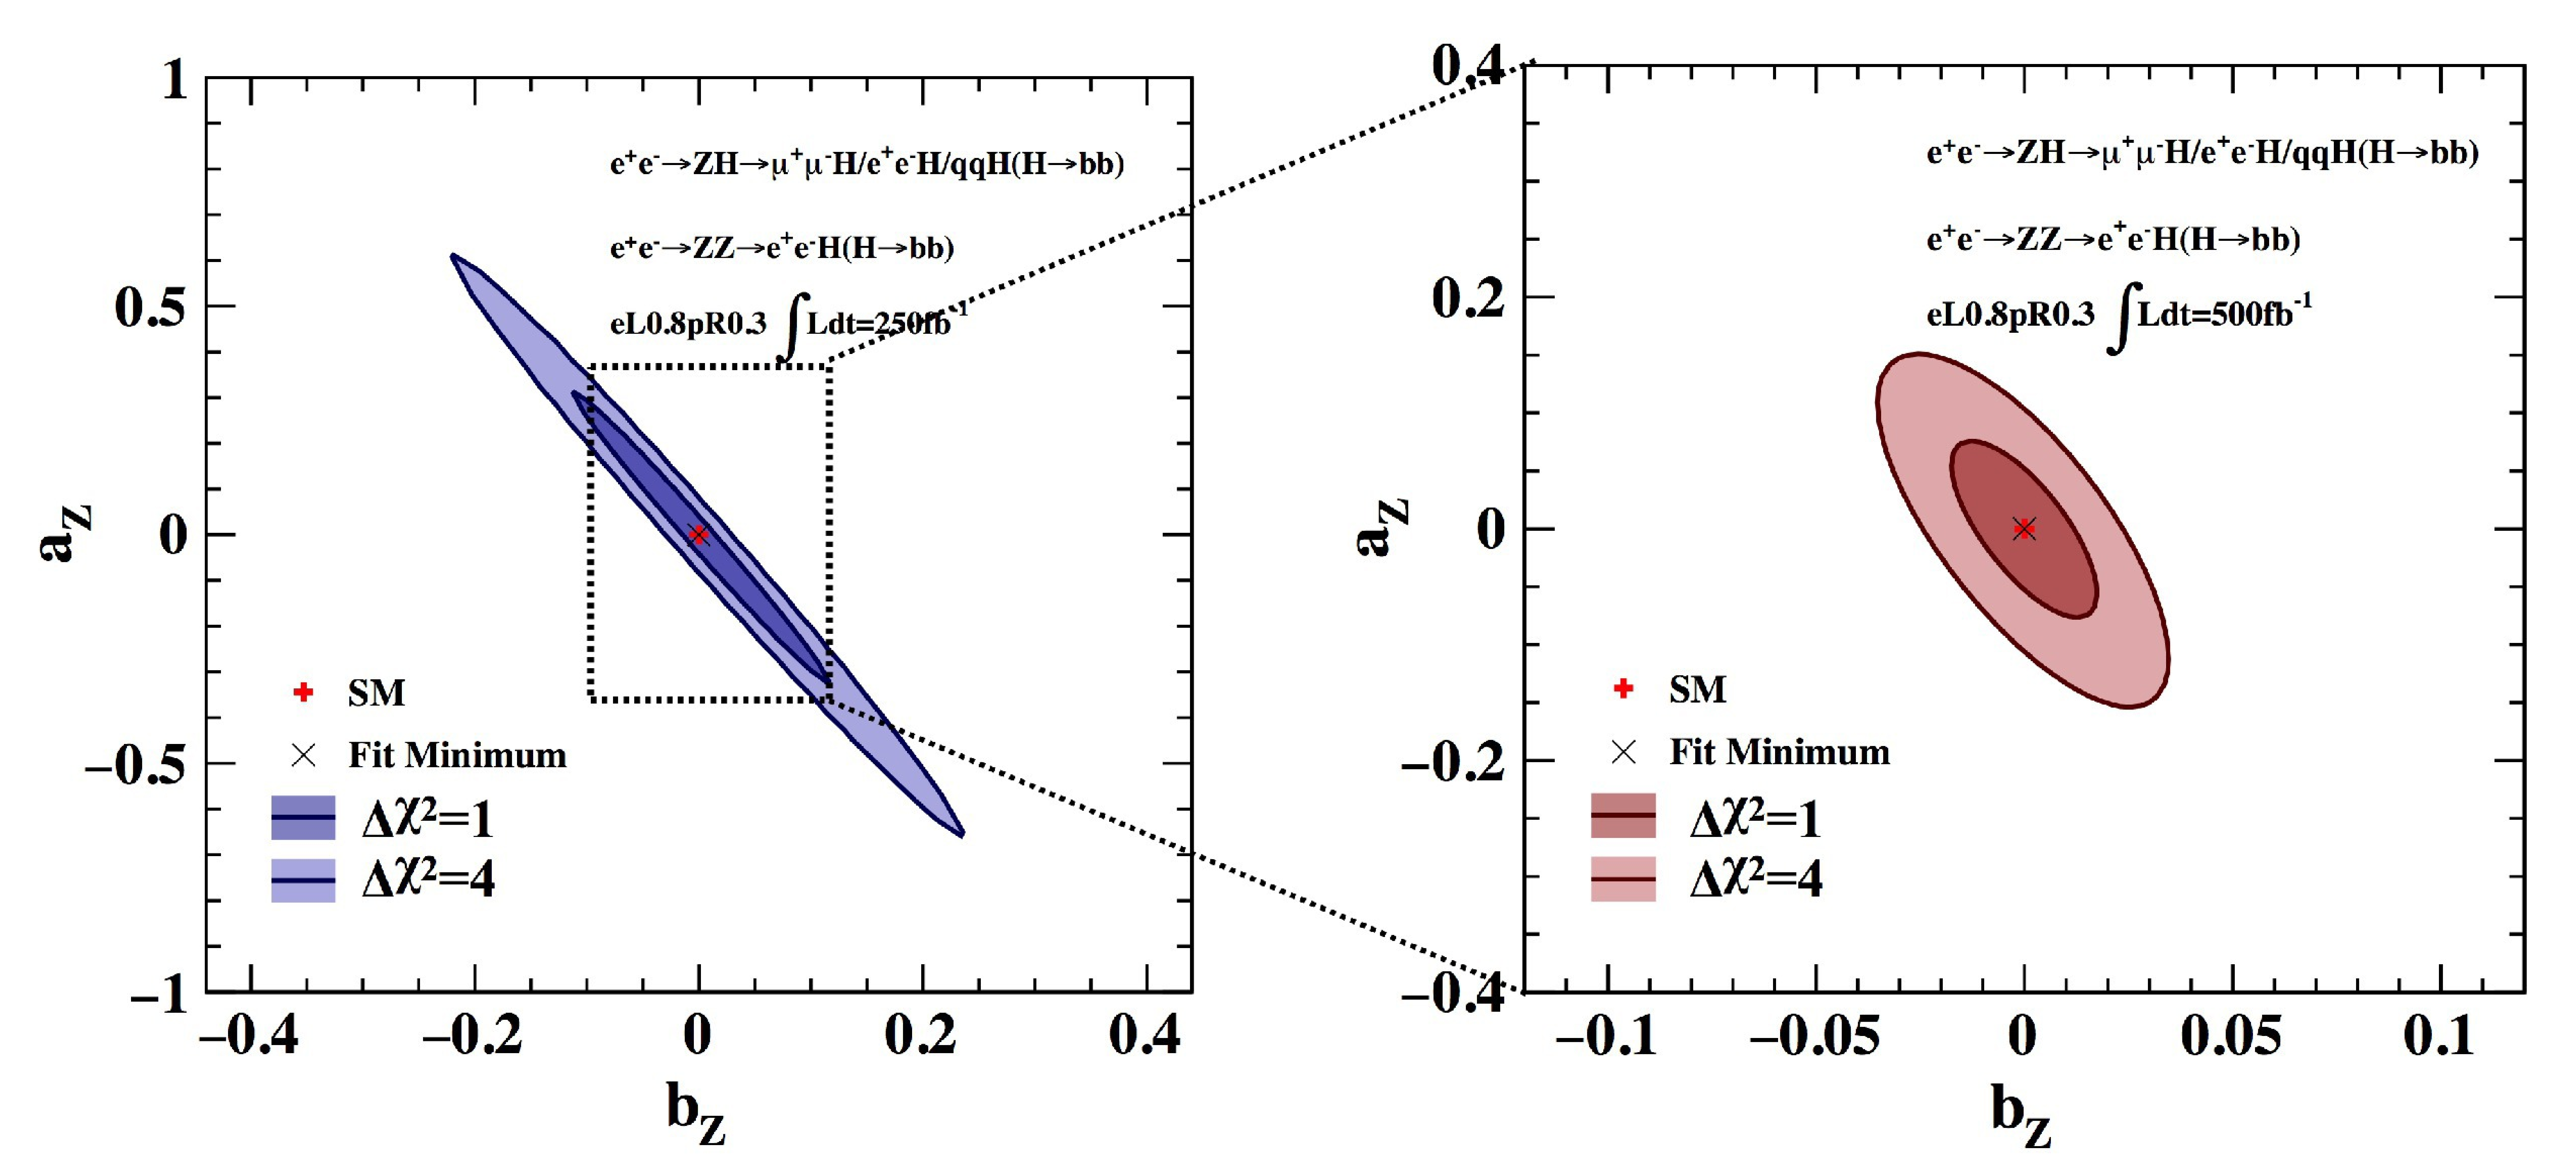
\includegraphics[width=0.85\hsize]{chapters/figures/ZH_anomHVV_ab.eps}
\end{center}
  \caption{68\% and 95\% C.L. contour plots for fitted parameter $a$ versus $b$ at 250 GeV (left)
  and 500 GeV (right);
  \cite{anomHVV}.}
  \label{fig:ZHanomHVV2}
\end{figure*}
